\section{Power-Law Hash Design and Implementation}
\label{sec:hash}

In key grouping operation, many grouping approaches need to spill part of kv-pairs to disk when the memory used has reached the threshold, these spilled partitions will be read back to re-aggregate subsequently. If the group sizes of data set follow a power-law distribution, 
it is more difficult for these approaches to divide the work data into small uniform portions, then several great partitions may be create if some big groups are spilled to the same portion. For a large partition spilled to disk, subsequent reading back and re-aggregating may lead to recursively execute the process many times when the memory is limited, the I/O overhead increases sharply. So we take the group size into account and propose to deal with the big groups and small groups separately. And we found that the indexing and filling method is suitable for big group key grouping, and the partitioned hash grouping is a good choice for small groups. For the data sets whose group sizes follow power-law distributions, the total size of big groups occupies the majority of the data sets but the number of big groups is minority, these properties of small groups are just the opposite, so this idea of processing separately is applicable for these data set and the powerhash algorithm is proposed. 

\subsection{Overview of Powerhash}%3.1
Depending on the core idea of power-law hash, our algorithm can be divided into three phases: Distinguishing, Indexing and Filling, Partitioned hash. The whole process is shown in Figure \ref{fig:pwHash}.
\begin{figure}
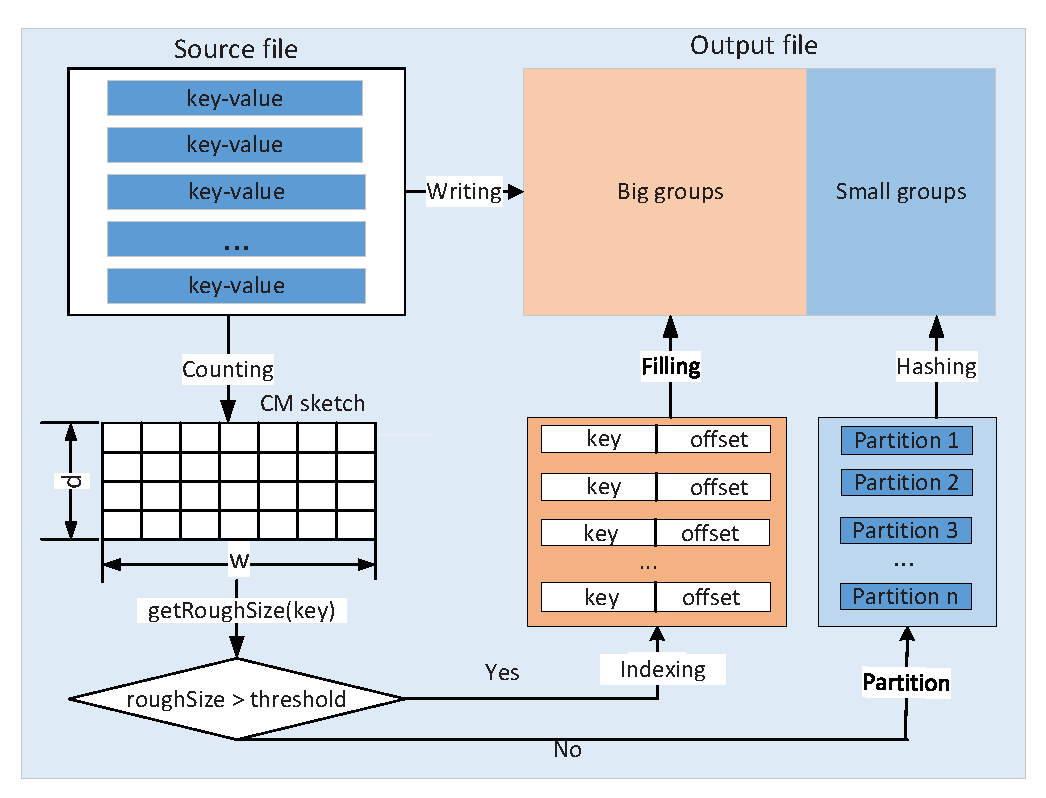
\includegraphics[width=.5\textwidth]{fig/pwhash}
\caption{Overview Intuition of Power-Law Hash.}
\label{fig:pwHash}
\end{figure}

Distinguishing phase is to distinguish between the big groups and small groups. First, it gets group sizes by the CM sktch, the distribution of group sizes is obtained at the same time, and it often follows a power-law distribution. Then, it distinguishes between the big groups and small groups based on their rough group size according to the Pateto principle. The CM sketch help us divide the big groups and small groups efficiently.

Indexing and Filling phase aims to group the kv-pairs in big groups, it generates an offset index that records the output positions of big groups firstly, and then fills the result file by file random access on the basis of the offset index. The output positions stored in the offset index are some integers, so the offset index size are much less than the hash table uesd to store kv-pairs in hash-based grouping methods, particularly for big groups. Each kv-pair does not need to store in memory and is written to the certain position in the result file directly, by which much repeat access to disk caused by out-of-memory can be avoided.

Partitioned hash phase is to group the kv-pairs in small groups. After grouping big groups, the small group sizes vary over a small range. This phase divides the small groups into several partitions through hashing, this division can avoid unbalanced partition to a great extent bacause big groups has been processed. Then, the kv-pairs in each partition are grouped by hashing on keys. If a partition is not fit in memory when hash grouping, the large partition will be redivided until its sub-partition can be processed in memory.

To reduce the cost of I/Os and improve the performance, we exploit an intermediate file to record the key and the value size information that is necessary for offset index generation, by which we can avoid to traverse the whole input file. In addition, an output buffer is used when grouping the kv-pairs. In the following, we describe the three phases in detail.

\subsection{Phase 1: Distinguishing}%3.1

The first phase is to distinguish between the big groups and small groups. As shown in Figure \ref{fig:pwHash}, an in-memory two-dimensional array is maintained to count the rough size for each group, it is the working process of CM sketch. The group size is how many bytes a group occupies. Because many data sets' group sizes follow power-law distributions, according to the Pareto principle, we can distinguish between the big groups and small groups depending on the rough group sizes, and then employ targeted methods to deal with the big groups and small groups, so the first phase is the basis of the whole algorithm. 

First, we need to obtain the group size of each group. The CM sketch can count the frequency of each distinct item in a data set quickly with small space if minor errors can be allowed. In our algorithm, the counting process is the accumulation of the kv-pairs' sizes(in bytes) as introduced in section \ref{sec:related}. Though the group sizes counted by CM sketch is inaccurate owing to the collisions of hashing, the CM sketch can ensure that the groups that are real big groups must have great statistical results and the groups with counting results must be real small groups.   
%those groups judged as small group are right and the big groups are not be judged as small groups, by which all big groups are identified accurately in spite of partial small groups are incorrectly identified as big groups. 

Then we need to judge which groups are big groups on the basis of the CM sketch where rough group sizes are stored. Because the data set's group sizes follow a power-law distribution, if we can know the ratio $r$ of big groups in the data set, the big groups and small groups can be divided easily. Referring to the Pareto principle(80/20 rule), the number of big groups only occupies aroud 20\% of the total groups but their total size takes up about 80\% of the total size, the ratio can be set around 0.2, the groups whose group sizes are the top 20\% in the data set are big groups, the rest are small groups. If we sort the whole group sizes, the big groups can be obtained, but the cost of sorting the whole group sizes is great, we need to traverse the input data set again and then sort the rough group sizes. Each row of the CM sketch is the counting result after passing the whole data set, we found that it can reflect the distribution of group sizes roughly, so we determine to sort one row of the CM sketch instead of sort all of group sizes. The width of CM sketch is $w$, if we sort a row of CM sketch in descending order, the threshold between big group sizes and small group sizes is the ${w*r}^{th}$ value. The groups whose rough group sizes are larger than the threshold are big groups. 

The whole distinguishing process can be completed efficiently by the employment of CM skech, its time cost occupies about 20\% of the total time according to experimental results.

\subsection{Phase 2: Indexing and Filling} 

Indexing and Filling phase is the grouping process of big groups. In the data sets whose group sizes follow the power-law distributions, the total size of big groups takes up about 80\% of the data set size according to the Pareto principle. If the big groups are processed by the hash-based grouping methods in limited memory, the hash table will be great. Once the hash table becomes too large to be fit in memory, the kv-pairs would be written to and then read from disk frequently, the repeat access to disk reduces the performance of key grouping. The I/O cost in key grouping with limited memory is reduced by the indexing and filling method in our algorithm, the property that the number of big groups only occupies aroud 20\% of the total groups makes it more feasible in limited memory, because the offset index will be smaller if the big groups are grouped separately in the whole process, and filling the output files with big groups will lead to relatively large amount of sequential writes but less number of seeks. 
%Indexing and Filling exploits the features of the file random access to complete the key grouping operation of big groups. 

Firstly, we need to structure an offset index that records the output positions of big groups. The offset here means the number of bytes from the written position of the group to the beginning of the file. With a specific output order, each big group's write-out position (i.e. offset) can be calculated, it is the accumulation of group sizes of all previous groups that has been accessed, so we need to count each big group's accurate size. The accurate group size is the accumulation of each kv-pair size(in byte). when a group is judged as a big group, the kv-pairs in the big group will be accumulated according to the unique $key$ of the group like Formula \ref{eq:accurate_size}.
\begin{equation}\label{eq:accurate_size}
    groupsize += sizeof(key) + sizeof(value)
\end{equation}
Each group size represents how many bytes the big group will take up in the final output file. With a specific output order, each offset is the
the accumulation of group sizes of all previous groups that has been accessed. If the big group sizes are stored in a group size table in $\langle key, groupsize\rangle$ format, we can get the group offsets while traversing the group size table, in which case the traversing order is the output order, i.e., the order of these big groups in the result file is the same with the traversing order. Based on the method, the $\langle key, groupsize\rangle$s are transformed to $\langle key, offset\rangle$s saved in the offset index as shown in Figure \ref{fig:convert}.

\begin{figure}
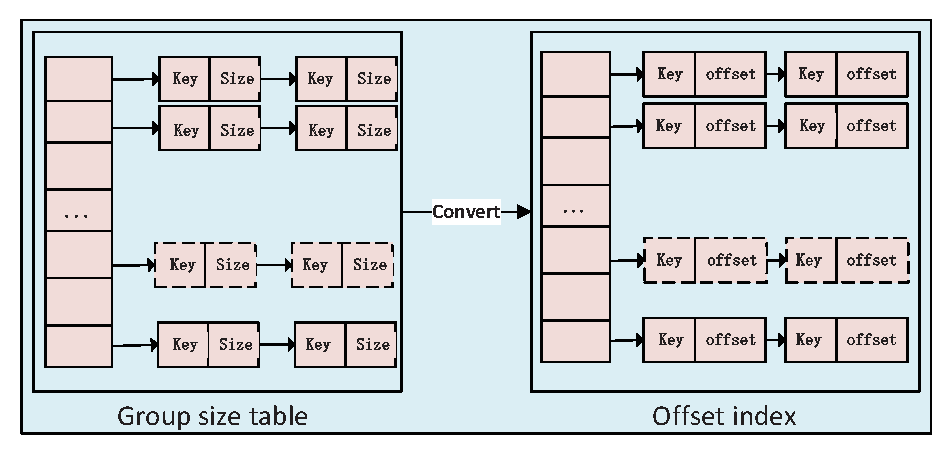
\includegraphics[width=.5\textwidth]{fig/convert}
\caption{The offset index generation.}
\label{fig:convert}
\end{figure}

Compared to the hash table in hash-based grouping methods, the offset index size is much less than the hash table where kv-pairs are stored, because the offset index only saves some integer --- the offsets---instead of storing kv-pairs. What's more, the big groups are processed separately in our algorithm, and the big groups are minority in the data sets, the space that the offset index occupies can be further reduce.
 
After constructing the offset index, the kv-pairs in big groups are written to the certain position in the result file depending on the corresponding offset. In the whole process, the big groups are not saved in memory in the whole group format, each kv-pair is read into memory and then written to the result file directly, only the offset index is always kept in memory, besides the necessay reading from and writing to the disk, there is no extra access to disk, so it can perform faster as shown in \ref{fig:paretoBig}. The profiling of this process shows that most of time is spent on seek operations during the file filling, this is mainly due to the fact that the writing of kv-pairs is not necessarily sequential, but filling the output files with big groups will lead to relatively large amount of sequential writes but less number of seeks.

\subsection{Phase 3: Partitioned Hash}

For a data set whose group sizes follow a power-law distribution, the majority of data set has been written to the result file after dealing with the big groups, the rest are small groups and the number of small groups are great than big groups, if we still employ indexing and filling method to group the kv-pairs in small groups, the size of offset index will increase a lot and may cause out-of-memory problem. In addition, the small group sizes vary over an small range, which can balanced division if we partition the small groups according to the available memory. In order to ensure the correctness of key grouping on small groups, the partition method we adopt is hashing, so we need to get the partition number, the partition number is determined by the available memory and the small groups number. 

For better analysis, we first define the following identifiers: the total size $T$ of data set, the current available memory $A$, the entry size $sizeof(entry)$ of the hash table used to grouping the small groups. In addition, the total size $S$ of small groups can be got after phase 1, the big group number $b$ can be obtained after phase 2. Combined with the ratio $r$ of big groups, the small group number $s$ is $b*(1-r)/r$. The space occupied when small groups are being processed is $S + sizeof(entry)*s$.
Because the actual hash table in small groups key grouping may be larger than the calculation, so we set an expansion factor $\alpha$ to expand the hash table size appropriately. So the partition number $P$ of small groups can be got like Formula \ref{eq:partition_num}. 
\begin{equation}\label{eq:partition_num}
    p = \dfrac{S + \alpha*sizeof(entry)*s}{A}
\end{equation}
For a kv-pair in a small groups, calculate the hash value $H_{key}$ first because the key may has various forms, and then hash the kv-pair to a partition depending on the partition id calculated by Formula \ref{eq:partition_hash}.
\begin{equation}\label{eq:partition_hash}
    id = H_{key} \%  p
\end{equation}  
Depending on the partition mode, the kv-pairs are hashed to different partitions, then the kv-pairs in small groups are grouped partition-by-partition by hash grouping method. Because the partition number is calculated roughly, the hash tables when dealing with several big parititions may be too large to be fit in memory, these great paritition will be divided into two parts and then be re-aggregated one-by-one, the repartition is an recursive process. Since the division is almost balanced, the repartition reduces a lot. Compared to the process of big groups, the partitioned hash grouping maintains the high performance of hashing grouping. Therefore, powerhash is an I/O efficient hash grouping approach with high performance in limited memory.  

\begin{algorithm}[ht]
    \caption{Power-Law Hash}
  \label{alg:group}
    \begin{algorithmic}[1]
    \Require  File \emph{F}, ratio \emph{r}, available memory \emph{A}, width \emph{w}, depth \emph{d}
    \Ensure result files $R$
    \State \emph{C:=} a two-dimensional array with width \emph{w} and depth \emph{d}
    \State \emph{H:=}\{\textbf{for} each \emph{i} \textbf{do} generate a hash function $h_i$, \emph{0 $\le$ i $\textless$d}\}    
    \State $key\_file :=$ a file of recording the key and value size
    \State initialize \emph{C = } \{\emph{C[$i$][$j$] = 0}, \emph{0 $\le$ i $\textless$d}, \emph{0 $\le$ j $\textless$ w} \}
    \For{each input $\langle key,value\rangle$ in \emph{F}}
    	\State write $\langle key,valuesize\rangle$ to the \emph{key\_file}
     	\For{ each $h_{i}() \in H $, \emph{0 $\le$ i $\textless$d} }
          \State \emph{C}[$i$][$h_{i}(key)$] += $sizeof(key) + sizeof(value)$
        \EndFor  
    \EndFor
    \State \emph{T:=} a group size table for the big groups
    \State calculate threshold \emph{t} between big groups and small groups.
    \For{each $\langle key,valuesize\rangle$ in \emph{key\_file}}
    	\State group size $f_{key}$ = \emph{min}(C[$i$][$h_{i}(key)$]), \emph{0 $\le$ i $\textless$d}
    	\If{ $f_{key} \textgreater$ \emph{t}}
    		\State insert the $\langle key,valuesize\rangle$ into \emph{T}    
    	\EndIf    	
    \EndFor
    \State calculte partition number \emph{p} depending on Fumula \ref{eq:partition_num}
    \State offset index $O:=Convert(T)$
    \State \emph{P:=} \{\textbf{for} each \emph{i} \textbf{do} generate a partition file $p_i$, \emph{0 $\le$ i $\textless$p}\}
    \For{ each input $\langle key,value\rangle$ in \emph{F}}
    	\If {there is a match in $O$ }
    		\State write the $\langle key,value\rangle$ into $R$
    		\State update the corresponding offset in $O$
    	\Else 
    		\State $id = H(key) \% p$
    		\State insert the $\langle key,value\rangle$ into $p_{id}$ 
    	\EndIf
    \EndFor
    \For{each $p_{id}$, \emph{0 $\le$ i $\textless$ p} }
		\State GroupBy($p_{id}$) in memory and Write to $R$
    \EndFor
    \State remove \emph{key\_file} and partition set \emph{P}
    \State output \emph{R}
    \end{algorithmic}
\end{algorithm}

\subsection{Algorithm analyse}
We summarize the whole process including the three phases in Algorithm \ref{alg:group}. The algorithm starts by creating a two-dimensional array with width \emph{w} and depth \emph{d} that is necessary to the CM sketch. Then each $\langle key, value\rangle$ pairs read from the input file \emph{F} is hashed to the CM sketch to calculate the rough size of each group. In order to avoid traversing the whole input file unnecessarily in phase 2, we use an intermediate file \emph{key\_file} to record the key and its corresponding value size in $\langle key, valuesize\rangle$ format during traversing the input file, i.e., we transform the original format $\langle key, value\rangle$ of the input data set into $\langle key, valuesize\rangle$ format, by which we can reduce the I/O cost and the computation of accurate group sizes in phase 2.

After counting the rough sizes, the threshold \emph{t} between the big groups and small groups is calculated depending on the CM sketch and the ratio $r$ of big groups(Line 12), we first sort one row of the two-dimensional array \emph{C} in descending order, the threshold \emph{t} is the ${d*r}^{th}$ element of the sorted row. While traversing the \emph{key\_file}, the $\langle key, valuesize\rangle$ belonging to big groups are insert to the group size table to calculate the accurate groug size like Formula \ref{eq:accurate_size}. The other $\langle key, valuesize\rangle$ pairs are accumulated to get the total size of small groups. We can get the group size table and other necessary factors after traversing the \emph{key\_file}, the partition number $p$ can be calculated like Formula \ref{eq:partition_num}, and offset index will be converted from the group size table.

The $Convert$ function converts the group size table to offset index (Line 22), in more details, traverses the elements in table $T$ from top to down and then accumulate the group sizes as the offset depending on the traversing order. The first entry of the table $T$(i.e. the first $\langle key, groupsize\rangle$) is the first group, so the initial offset of the entry equals to 0, it means that the first kv-pair mapped to the group will be stored in the beginning of the result file. Define the group size of the previous entry as $group_{pre}$, which means that the size of the previous group is $group_{pre}$. Define the initial offset of the previous group as ${off}_{pre}$. So the offset of current entry ${off}_{cur}$ equals to the sum of ${off}_{pre}$ and $group_{pre}$. After calculate the offset of each group, we will obtain an in-memory offset index which contains $\langle key,offset\rangle$ information. 

Finally, filling the result file phase needs another pass of the input file, the kv-pairs in big groups are written to the result file in terms of the offset index(see lines 22-25 in Algorithm \ref{alg:group}). For a kv-pair, get the offset ${off}_{key}$  by searching the offset index $O$, if there is a match in the index, it belongs to a big group and will be written to the ${off}^{th}_{key}$ bytes of the result file \emph{R} depending on the offset, if there is no match, it will be written to the corresponding partition in \emph{P}. With a kv-pair from input file having been output, the current offset of the corresponding group will increase the size of the kv-pair in bytes, which indicates the next kv-pair mapped to the same group will be stored in the ${({off}_{cur} + sizeof(\langle key,value\rangle ))}^{th}$ bytes of the file \emph{R}. It is the update operation in line 25 of Algorithm \ref{alg:group}.

After grouping the big groups successfully, the small group in each partitions stored in the disk are still unordered, these small group partitions are read into memory partition-by-partition and processed by the hash grouping, then these kv-pairs in small group partitions are appended to the result file \emph{R} after grouping(as shown 31-33 in algorithm \ref{alg:group}). 






